\documentclass[a4paper]{article}

% 文章排版
\usepackage{indentfirst}
\setlength{\parindent}{0em}
\usepackage{autobreak}
\allowdisplaybreaks
\usepackage{parskip}
\usepackage{geometry}
\geometry{top=3cm,bottom=3cm,left=2cm,right=2cm}
\usepackage{anyfontsize}

% 数学物理宏包
\usepackage{amsmath,amssymb}
\usepackage{tabularray}
\UseTblrLibrary{amsmath}
\usepackage{physics}
\renewcommand\div\divisionsymbol
\DeclareMathOperator{\diag}{diag}
\newcommand{\trans}{\text{\textsf{T}}}

\usepackage{fontspec}
\setmainfont{Lucida Bright OT}
\usepackage{unicode-math}
\unimathsetup{mathrm=sym,mathbf=sym,mathsf=sym,math-style=ISO,bold-style=ISO}
\setmathfont[StylisticSet=4,sans-style=italic]{Lucida Bright Math OT}
\setmathfont[range={\mathscr,\mathbfscr}]{Lucida Bright Math OT}

\usepackage[fontset=none]{ctex}
\setCJKmainfont{FZShuSong-Z01}[BoldFont=Source Han Sans CN,ItalicFont=FZKai-Z03]
\setCJKsansfont{Source Han Sans CN}
\usepackage{tikz}
\usetikzlibrary{arrows.meta}
\usetikzlibrary{decorations.pathmorphing}
\usetikzlibrary{decorations.pathreplacing}

% 符号重定义
\AtBeginDocument{
    \let\uglyepsilon\epsilon
    \renewcommand\epsilon\varepsilon
    \let\uglyleq\leq
    \renewcommand\leq\leqslant
    \let\uglygeq\geq
    \renewcommand\geq\geqslant
}


% 题目
\title{\textbf{广义相对论\ \ \ \ 第一次作业}}
\author{张植竣 1900011604}
\date{2023年3月20日}

\begin{document}

\maketitle

\section*{第一章}

\begin{enumerate}
    \item[9.]
    记发射器的4-速度为$\hat{u}_e$，观测者的4-速度为$\hat{u}_o$，光子的4-动量为$\hat{p}$。

    则发射光子的能量为$E_e = -\hat{p} \cdot \hat{u_e}$，观测到光子的能量为$E_o = -\hat{p} \cdot \hat{u}_o$

    于是有：
    \[
        \frac{\lambda_o}{\lambda_e} = \frac{E_e}{E_o} = \frac{-\hat{p} \cdot \hat{u_e}}{-\hat{p} \cdot \hat{u_o}} = \frac{p^0 u_e^0 - \mathbf{p} \cdot \mathbf{u}_e}{p^0 u_e^0 - \mathbf{p} \cdot \mathbf{u}_e}
    \]

    由于发射器在圆心，相对于地面静止，$\mathbf{u}_e = 0$，即$\hat{u}_e = (1,\ 0,\ 0,\ 0)$，则有：
    \[
        p^0 u_e^0 - \mathbf{p} \cdot \mathbf{u}_e = p^0
    \]
    又因为圆盘做匀角速度运动，圆盘边缘观测者速度大小为$|\mathbf{u}_o| = v$。速度沿切线方向，与$\mathbf{p}$垂直，则$\hat{u}_o = \gamma(1,\ \mathbf{v})$，且：
    \[
        p^0 u_o^0 - \mathbf{p} \cdot \mathbf{u}_o = \gamma p^0
    \]
    故：
    \[
        \frac{\lambda_o}{\lambda_e} = \frac{p^0}{\gamma p^0} = \frac{1}{\gamma} = \sqrt{1 - v^2} < 1
    \]
    根据红移因子$z$的定义：
    \[
        z = \frac{\lambda_o - \lambda_e}{\lambda_e} = \sqrt{1 - v^2} - 1 < 0
    \]
    即圆盘便越观测者接收到原点发出的光子波长变短，被蓝移。

    \bigskip
    \item[10.]
    不妨设4-速度为$\hat{u}_1$的飞船为观测者。在观测者实验室中，观测者自身的4-速度为$\hat{u} = (1,\ 0,\ 0,\ 0)$，另一艘飞船的相对4-速度为$\hat{u}_r = \gamma(1,\ \mathbf{v})$。

    于是有：
    \[
        \hat{u}_1 \cdot \hat{u_2} = \hat{u} \cdot \hat{u}_r = \eta_{00} u^0 u_r^0 = -\gamma
    \]
    即：
    \[
        (\hat{u}_1 \cdot \hat{u_2})^2 = (-\gamma)^2 = \frac{1}{1 - v^2}
    \]
    则有：
    \[
        v^2 = \frac{(\hat{u}_1 \cdot \hat{u_2})^2 - 1}{(\hat{u}_1 \cdot \hat{u_2})^2}
    \]

    \bigskip
    \item[15.]
    如图，设地面系为$\varSigma$系，平面镜的静止参考系为$\varSigma'$系，入射波矢为$\mathbf{k}_i$，反射波矢为$\mathbf{k}_o$。

    \begin{center}
    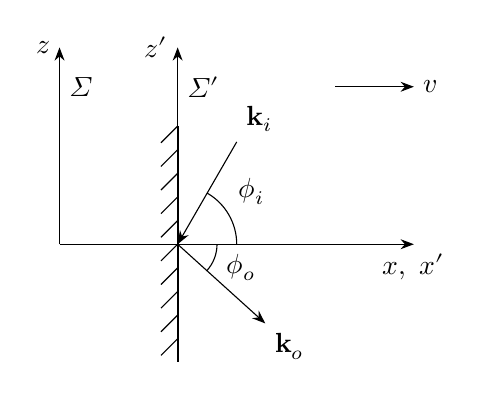
\begin{tikzpicture}[decoration={border,segment length=3mm,angle=-45,amplitude=3mm},>=Stealth]
        \draw [->] (-1.5,0) -- (3,0) node [below] {$x,\ x'$};
        \draw [->] (-1.5,0) -- (-1.5,2.5) node [left] {$z$};
        \draw [->] (0,0) -- (0,2.5) node [left] {$z'$};
        \draw [->] (2,2) -- (3,2) node [right] {$v$};
        \draw (-1.5,2) node [right] {$\varSigma$};
        \draw (0,2) node [right] {$\varSigma'$};
        \draw [thick] (0,1.5) -- (0,-1.5);
        \draw [decorate] (0,1.5) -- (0,-1.5);
        \draw [->] (0.75,1.2990381) -- (0,0) node [at start, anchor=south west] {$\mathbf{k}_i$};
        \draw [->] (0,0) -- (1.1129032,-1.0057069) node [anchor=north west] {$\mathbf{k}_o$};
        \draw (0.75,0) arc [start angle=0,end angle=60,radius=0.75] node [midway,anchor=south west] {$\phi_i$};
        \draw (0.5,0) arc [start angle=0,end angle=-42.1034489,radius=0.5] node [at start,anchor=north west] {$\phi_o$};
    \end{tikzpicture}
    \end{center}

    在$\varSigma$系中，入射波的4-波矢为：
    \[
    \hat{k}_i = (\omega_i,\ \mathbf{k}_i) = \qty(-\omega_i\cos\phi_i,\ 0,\ -\omega_i\sin\phi_i,\ \omega_i)
    \]
    参考系$\varSigma'$与$\varSigma$之间的4-波矢变换为：
    \[
    k'_x = \gamma\qty(k_x-\beta\frac{\omega}{c}),\quad k'_y = k_y,\quad k'_z = k_z,\quad \frac{\omega'}{c} = \gamma\qty(\frac{\omega}{c}-\beta k_x)
    \]
    则在$\varSigma'$系中，入射波的4-波矢为：
    \[
    \hat{k}'_i = (\omega_i,\ \mathbf{k}_i) = \qty(-\gamma\omega_i (\beta+\cos\phi_i),\ 0,\ -\omega_i\sin\phi_i,\ \gamma\omega_i (1+\beta\cos\phi_i))
    \]
    在$\varSigma'$系中，入射角等于反射角，入射波与反射波频率相等，则反射波的4-波矢为：
    \[
    \hat{k}'_o = \qty(k'_x,\ k'_y,\ k'_z,\ \frac{\omega'_o}{c}) = \qty(\gamma\omega_i (\beta+\cos\phi_i),\ 0,\ -\omega_i\sin\phi_i,\ \gamma\omega_i (1+\beta\cos\phi_i))
    \]
    参考系$\varSigma$与$\varSigma'$之间的4-波矢变换为：
    \[
    k_x = \gamma\qty(k_x' + \beta\frac{\omega'}{c}),\quad k_y = k_y',\quad k_z = k_z',\quad \frac{\omega}{c} = \gamma\qty(\frac{\omega'}{c} + \beta k'_x)
    \]
    则在$\varSigma$系中，反射波的4-波矢为：
    \[
    \hat{k}_o = \qty(\gamma^2\omega_i\qty(\cos\phi_i+2\beta+\beta^2\cos\phi_i),\ 0,\ -\omega_i\sin\phi_i,\ \gamma^2\omega_i\qty(1+2\beta\cos\phi_i+\beta^2))
    \]
    于是有：
    \[
    \omega_o = \gamma^2\omega_i\qty(1+2\beta\cos\phi_i+\beta^2)
    \]
    由$\gamma=\dfrac{1}{\sqrt{1-\beta^2}}$得：
    \begin{equation}
        \omega_o = \omega_i \frac{1 + 2\beta\cos\phi_i + \beta^2}{1-\beta^2}
    \end{equation}
    首先有：
    \begin{equation}
    \tan\phi_o = \frac{-k_{oz}}{k_{ox}} = \frac{\sin\phi_i}{\gamma^2\qty(\cos\phi_i+2\beta+\beta^2\cos\phi_i)} = \frac{\qty(1-\beta^2)\sin\phi_i}{\cos\phi_i + 2\beta + \beta^2\cos\phi_i}
    \end{equation}
    或由$k_o=\dfrac{\omega_o}{c}\cos\phi_o$得：
    \begin{equation}
    \cos\phi_o = \frac{\cos\phi_i + 2\beta + \beta^2\cos\phi_i}{1 + 2\beta\cos\phi_i + \beta^2}
    \end{equation}
    将(2)、(3)两式相乘得：
    \begin{equation}
        \sin\phi_o = \frac{1 - \beta^2}{1 + 2\beta\cos\phi_i + \beta^2} \sin\phi_i
    \end{equation}
    与(1)式联立得：
    \[
        \frac{\nu_o}{\nu_i} = \frac{\sin\phi_i}{\sin\phi_o}
    \]
    另一方面，注意到$\tan(\alpha/2) = \dfrac{\sin\alpha}{1 + \cos\alpha}$，则由(3)式得：
    \[
        1 + \cos\phi_o = \frac{(1+\beta)^2 (1+\cos\phi_i)}{1 + 2\beta\cos\phi_i + \beta^2}
    \]
    与(4)式联立得：
    \[
        \frac{\sin\phi_o}{1 + \cos\phi_o} = \frac{(1 - \beta) (1 + \beta)}{(1+\beta)^2 (1+\cos\phi_i)} = \qty(\frac{1 - \beta}{1 + \beta}) \frac{\sin\phi_i}{1 + \cos\phi_i}
    \]
    即：
    \[
        \frac{\tan(\phi_i/2)}{\tan(\phi_o/2)} = \frac{1 + \beta}{1 - \beta} = \frac{c + v}{c - v}
    \]
\end{enumerate}

\clearpage
\section*{第二章}

\begin{enumerate}
    \item[1.]
    由题意得：
    \begin{align*}
        \epsilon_{\alpha\beta\gamma\delta} \eta^{\alpha\mu} \eta^{\beta\nu} \eta^{\gamma\rho} \eta^{\delta\lambda} \epsilon_{\mu\nu\rho\lambda}
        &= \epsilon_{\alpha\beta\gamma\delta} \eta^{\alpha\mu} \eta^{\beta\nu} \eta^{\gamma\rho} \epsilon_{\mu\nu\rho}^{\ \ \ \ \delta} \\
        &= \epsilon_{\alpha\beta\gamma\delta} \eta^{\alpha\mu} \eta^{\beta\nu} \epsilon_{\mu\nu}^{\ \ \ \gamma\delta} \\
        &= \epsilon_{\alpha\beta\gamma\delta} \eta^{\alpha\mu} \epsilon_\mu^{\ \beta\gamma\delta} \\
        &= \epsilon_{\alpha\beta\gamma\delta} \epsilon^{\alpha\beta\gamma\delta}
    \end{align*}
    最后只需要计算Levi-Civita完全反对称张量的完全收缩。

    在闵可夫斯基时空下，采用常见的约定$\epsilon_{0123}=+1$ 且以度规$\eta_{\mu\nu}=\diag(-,+,+,+)$为准时：
    \[
    \epsilon_{\alpha\beta\gamma\delta} \epsilon^{\alpha\beta\gamma\delta} = -1 \times 4! = -24
    \]
    推导如下：

    首先通过升指标得到：
    \[
        \epsilon^{\alpha\beta\gamma\delta} = \eta^{\alpha\alpha'}\eta^{\beta\beta'}\eta^{\gamma\gamma'}\eta^{\delta\delta'} \epsilon_{\alpha'\beta'\gamma'\delta'}
    \]
    一般规定$\epsilon^{0123} = +1$，对闵氏度规 $\eta = \diag(-,+,+,+)$有：
    \[
        \epsilon^{0123}=\eta^{00}\eta^{11}\eta^{22}\eta^{33}\,\epsilon_{0123} = -1 \times \epsilon_{0123} = -1
    \]
    $\epsilon_{\alpha\beta\gamma\delta}$在任意有重复索引时为 0，非零项只出现在所有$4!$个对0、1、2、3的不同的排列上，而对任意排列$\pi$，有：
    \[
        \epsilon_{\pi} \epsilon^{\pi} = -1 \times (\epsilon_\pi)^2 = -1
    \]
    共有$4! = 24$个非零排列项，每项值均为$-1$，所以求和后为：
    \[
    \epsilon_{\alpha\beta\gamma\delta}\epsilon^{\alpha\beta\gamma\delta} = 4! \times (-1) = -24
    \]
    推广地，如果在一个$n$维空间中，度规为对角矩阵，其中有$s$个$-1$和$n-s$个$+1$，则：
    \[
    \epsilon_{\mu_1\ldots\mu_n} \epsilon^{\mu_1\ldots\mu_n} = n! (-1)^s
    \]

    \bigskip
    \item[2.]
    令张量$X^{\mu\nu}$的矩阵表示为：
    \[
        \mathsf{X} =
        \begin{bmatrix}
            1 & -1 & 0 & 0 \\
            -1 & 0 & 5 & 3 \\
            -2 & 1 & 0 & 0 \\
            0 & 1 & 0 & 2
        \end{bmatrix}
    \]
    $V^\mu$的向量表示为$\mathsf{V} = (0,3,1,-2)^\trans$，$\eta_{\mu\nu}$的矩阵表示为$\mathsf{\eta} = \diag{(-1,1,1,1)}$，$\eta^{\mu\nu}$的矩阵表示为$\mathsf{\eta}^{-1} = \diag{(-1,1,1,1)}$。根据张量和矩阵的计算规则，有：
    \begin{enumerate}
        \item[(a)]
        缩并降第二个指标相当于右乘$\mathsf{\eta}$，只改变第一列的符号：
        \[
        X^\mu_{\ \nu} = X^{\mu\rho} \eta_{\rho\nu} = \mathsf{X \eta} =
        \begin{bmatrix}
            -1 & -1 & 0 & 0 \\
            1 & 0 & 5 & 3 \\
            2 & 1 & 0 & 0 \\
            0 & 1 & 0 & 2
        \end{bmatrix}
        \]

        \item[(b)]
        缩并降第一个指标相当于左乘$\mathsf{\eta}$，只改变第一行的符号：
        \[
        X_\mu^{\ \nu} = \eta_{\mu\rho} X^{\rho\nu} = \mathsf{\eta X} =
        \begin{bmatrix}
            -1 & 1 & 0 & 0 \\
            -1 & 0 & 5 & 3 \\
            -2 & 1 & 0 & 0 \\
            0 & 1 & 0 & 2
        \end{bmatrix}
        \]

        \item[(c)]
        交换两个指标相当于矩阵的转置：
        \[
        X^{(\mu\nu)} = \frac{1}{2}(X^{\mu\nu} + X^{\nu\mu}) = \frac{1}{2} (\mathsf{X} + \mathsf{X}^\trans) =
        \begin{bmatrix}
            -1 & -1 & 0 & 0 \\
            1 & 0 & 5 & 3 \\
            2 & 1 & 0 & 0 \\
            0 & 1 & 0 & 2
        \end{bmatrix}
        \]

        \item[(d)]
        缩并升两个指标相当于左乘和右乘$\mathsf{\eta}$：
        \[
            X_{\mu\nu} = \eta_{\mu\rho} X^{\rho\sigma} \eta_{\sigma\nu} = \mathsf{\eta X \eta} =
        \begin{bmatrix}
            1 & 1 & 0 & 0 \\
            1 & 0 & 5 & 3 \\
            2 & 1 & 0 & 0 \\
            0 & 1 & 0 & 2
        \end{bmatrix}
        \]
        再计算反对称部分：
        \[
            X_{[\mu\nu]} = \frac{1}{2}(X_{\mu\nu} - X_{\nu\mu}) = \frac{1}{2} \qty[\mathsf{\eta X \eta} - (\mathsf{\eta X \eta})^\trans] =
        \begin{bmatrix}
            0 & 0 & -1 & 0 \\
            0 & 0 & 2 & 1 \\
            1 & -2 & 0 & 0 \\
            0 & -1 & 0 & 0
        \end{bmatrix}
        \]

        \item[(e)]
        张量求迹相当于矩阵求迹，但需要先转化为(1,1)-型张量：
        \[
            X^\lambda_\lambda = \tr(X^\mu_\nu) = \tr(X^{\mu\rho} \eta_{\rho\nu}) = \tr(\mathsf{X \eta}) = -1 + 0 + 0 + 2 = 1
        \]

        \item[(f)]
        一阶张量的内积相当于向量的内积，但需要先用度规张量将一个向量降指标：
        \[
            V^\mu V_\mu = V^\mu \eta_{\mu\nu} V^\nu = \mathsf{V^\trans \eta V} = (-1) \times 0^2 + 3^2 + 1^2 + (-2)^2 = 14
        \]

        \item[(g)]
        根据矩阵乘法的定义，要将矩阵$\mathsf{X}$的列与$\mathsf{V}$的每一个元素相乘再相加，即：
        \[
            V_\mu X^{\mu\nu} = W^\nu,\quad (W^\nu)_i = \sum_j V_j X^{ji}
        \]
        对应的矩阵/向量表示为：
        \[
            V_\nu X^{\mu\nu} = X^{\mu\nu} \eta_{\nu\rho} V^\rho = \mathsf{X^\trans \eta V} = (-5, -1, 15, 5)^\trans
        \]
        另一种算法是：
        \[
            V_\nu X^{\mu\nu} = \eta_{\nu\rho} V^\rho X^{\mu\nu} = \mathsf{(\eta V)^\trans X} = (-5, -1, 15, 5)
        \]
        这样得到的结果是一个行向量。
    \end{enumerate}

    \bigskip
    \item[11.(a)]
    对于Maxwell理论，首先写出电磁场张量$F_{\mu\nu}$的分量形式：
    \[
        F_{\mu\nu} =
        \begin{bmatrix}
        0 & -E_x & -E_y & -E_z \\
        E_x & 0 & B_z & -B_y \\
        E_y & -B_z & 0 & B_x \\
        E_z & B_y & -B_x & 0
        \end{bmatrix}
    \]
    其对应的(2,0)-型张量$F^{\mu\nu}$的分量形式为：（电场部分符号相反，磁场部分不变）
    \[
        F^{\mu\nu} = \eta^{\mu\alpha} \eta^{\nu\beta} F_{\alpha\beta} =
        \begin{bmatrix}
        0 & E_x & E_y & E_z \\
        -E_x & 0 & B_z & -B_y \\
        -E_y & -B_z & 0 & B_x \\
        -E_z & B_y & -B_x & 0
        \end{bmatrix}
    \]
    这给出：（两矩阵对应元素相乘再求和）
    \[
        F^{\mu\nu} F_{\mu\nu} = -2(E_x^2 + E_y^2 + E_z^2) + 2(B_x^2 + B_y^2 + B_z^2) = 2(B^2 - E^2)
    \]
    $F_{\mu\nu}$对应的(1,1)-型张量$F^\mu_{\ \nu}$的分量形式为：（只改变第一列的符号）
    \[
        F^\mu_{\ \nu} = \eta^{\mu\alpha} F_{\alpha\nu} =
        \begin{bmatrix}
        0 & E_x & E_y & E_z \\
        E_x & 0 & B_z & -B_y \\
        E_y & -B_z & 0 & B_x \\
        E_z & B_y & -B_x & 0
        \end{bmatrix}
    \]
    而$F^{\mu\lambda} F^\nu_{\ \lambda}$是一个二阶张量$G^{\mu\nu}$，它的每一个分量满足：
    \[
        G^{ij} = \sum_\lambda F^{i\lambda} F^j_{\ \lambda}
    \]
    这相当于矩阵$\mathsf{F^{\mu\nu}}$与矩阵$\mathsf{F^\mu_{\ \nu}}$转置的乘积：
    \[
        \mathsf{G} = \mathsf{F^{\mu\nu} (F^\mu_{\ \nu})^\trans}
    \]
    需要分类讨论如下：
    \begin{enumerate}
        \item[(1)]
        $i = j = 0$时：
        \[
            G^{00} = \sum_\lambda F^{0\lambda} F^0_{\ \lambda} = -E_x^2 - E_y^2 - E_z^2 = -E^2
        \]
        \item[(2)]
        $i = 0$，$j \neq 0$时：
        \[
            G^{0j} = \sum_\lambda F^{0\lambda} F^j_{\ \lambda} = E_x F^j_{\ 1} + E_y F^j_{\ 2} + E_z F^j_{\ 3} = (\mathbf{E} \times \mathbf{B})_j
        \]
        例如当$j = 1$时：
        \[
            G^{01} = E_x F^1_{\ 1} + E_y F^1_{\ 2} + E_z F^1_{\ 3} = 0 + E_y B_z - E_z B_y = (\mathbf{E} \times \mathbf{B})_x
        \]
        同理：
        \[
            G^{02} = E_z B_x - E_x B_z = (\mathbf{E} \times \mathbf{B})_y,\quad G^{03} = E_x B_y - E_y B_x = (\mathbf{E} \times \mathbf{B})_z
        \]
        因此：
        \[
            G^{0j} = (\mathbf{E} \times \mathbf{B})_j
        \]
        \item[(3)]
        $i \neq 0$，$j = 0$时，和上一种情况同理：
        \[
            G^{i0} = \sum_\lambda F^{i\lambda} F^0_{\ \lambda} = F^{i1} E_x + F^{i2} E_y + F^{i3} E_z = -(\mathbf{E} \times \mathbf{B})_i
        \]
        \item[(4)]
        $i \neq 0$，$j \neq 0$时：
        \[
            G^{ij} = \sum_\lambda F^{i\lambda} F^j_{\ \lambda} = F^{i0} F^j_{\ 0} + F^{ik} F^j_{\ k} = -E_i E_j + \sum_k F^{ik} F^j_{\ k}
        \]
        其中$k = 1,2,3$且$k \neq i$。需要分类讨论如下：
        \begin{enumerate}
            \item[(a)]
            $i = j$时：
            \[
                G^{ii} = -E_i^2 + \sum_{k \neq i} F^{ik} F^i_{\ k} = -E_i^2 + B^2 - B_i^2
            \]
            例如当$i = 1$时：
            \[
                G^{11} = -E_x^2 + F^{12} F^1_{\ 2} + F^{13} F^1_{\ 3} = -E_x^2 + B_z^2 + B_y^2 = -E_x^2 + B^2 - B_x^2
            \]
            同理：
            \[
                G^{22} = -E_y^2 + B^2 - B_y^2,\quad G^{33} = -E_z^2 + B^2 - B_z^2
            \]
            因此：
            \[
                G^{ii} = -E_i^2 + B^2 - B_i^2
            \]
            \item[(b)]
            $i \neq j$时：
            \[
                G^{ij} = E_i E_j + \sum_k F^{ik} F^j_{\ k} = E_i E_j + F^{ik} F^j_{\ k}
            \]
            其中$k = 1,2,3$且$k \neq i$且$k \neq j$，即求和号内$k$只有一个取值。

            例如当$(i,j) = (1,2)$时，$k = 3$，则有：
            \[
                G^{12} = -E_x E_y + F^{13} F^2_{\ 3} = E_x E_y - B_y B_x
            \]
            同理可得：
            \[
                G^{ij} = -E_i E_j - B_i B_j,\quad (k \neq i,\ k \neq j)
            \]
        \end{enumerate}
        则$i \neq 0$，$j \neq 0$时，$G^{ij}$可以统一写为：
        \[
            G^{ij} = \sigma_{ij} = -E_i E_j + (B^2 \delta_{ij} - B_i B_j)
        \]
        也可以用如下方法证明：
        \[
            F^{ik}F^j_{\ k} = F^{ik}F^{jk} = (-\epsilon_{ikm} B^m)(-\epsilon_{jkn} B^n) = \epsilon_{ikm} \epsilon_{jkn} B^m B^n
        \]
        又因为：
        \[
            \epsilon_{ikm} \epsilon_{jkn} = \delta_{ij} \delta_{mn} - \delta_{in} \delta_{jm}
        \]
        则有：
        \[
            F^{ik}F^j_{\ k} = (\delta_{ij} \delta_{mn} - \delta_{in} \delta_{jm}) B^m B^n = \delta_{ij}(\delta_{mn} B^m B^n) - \delta_{in}B^n (\delta_{jm} B^m) = B^2 \delta_{ij} - B_i B_j
        \]
    \end{enumerate}
    综上所述，$G^{\mu\nu}$的分量形式为：
    \[
        G^{\mu\nu} =
        \begin{bmatrix}
        -E^2 & (\mathbf{E} \times \mathbf{B})_x & (\mathbf{E} \times \mathbf{B})_y & (\mathbf{E} \times \mathbf{B})_z \\
        -(\mathbf{E} \times \mathbf{B})_x & \sigma_{xx} & \sigma_{xy} & \sigma_{xz} \\
        -(\mathbf{E} \times \mathbf{B})_y & \sigma_{yx} & \sigma_{yy} & \sigma_{yz} \\
        -(\mathbf{E} \times \mathbf{B})_z & \sigma_{zx} & \sigma_{zy} & \sigma_{zz}
        \end{bmatrix}
    \]
    其中：
    \[
        \sigma_{ij} = B^2 \delta_{ij} - (E_i E_j + B_i B_j)
    \]
    于是我们可以写出$T_{\mathrm{EM}}^{\mu\nu}$为：
    \begin{align*}
        T_{\mathrm{EM}}^{\mu\nu}
        &= F^{\mu\lambda} F^\nu_{\ \lambda} - \frac{1}{4} \eta^{\mu\nu} F^{\alpha\beta} F_{\alpha\beta} \\
        &= G^{\mu\nu} - \frac{1}{2} \eta^{\mu\nu} (B^2 - E^2) \\
        &= \begin{bmatrix}
        (E^2 + B^2)/2 & (\mathbf{E} \times \mathbf{B})_x & (\mathbf{E} \times \mathbf{B})_y & (\mathbf{E} \times \mathbf{B})_z \\
        -(\mathbf{E} \times \mathbf{B})_x & \sigma_{xx} - (E^2 + B^2)/2 & \sigma_{xy} & \sigma_{xz} \\
        -(\mathbf{E} \times \mathbf{B})_y & \sigma_{yx} & \sigma_{yy} - (E^2 + B^2)/2 & \sigma_{yz} \\
        -(\mathbf{E} \times \mathbf{B})_z & \sigma_{zx} & \sigma_{zy} & \sigma_{zz} - (E^2 + B^2)/2
        \end{bmatrix} \\
        &= \begin{bmatrix}
        (E^2 + B^2)/2 & (\mathbf{E} \times \mathbf{B})_x & (\mathbf{E} \times \mathbf{B})_y & (\mathbf{E} \times \mathbf{B})_z \\
        -(\mathbf{E} \times \mathbf{B})_x & \tau_{xx} & \tau_{xy} & \tau_{xz} \\
        -(\mathbf{E} \times \mathbf{B})_y & \tau_{yx} & \tau_{yy} & \tau_{yz} \\
        -(\mathbf{E} \times \mathbf{B})_z & \tau_{zx} & \tau_{zy} & \tau_{zz}
        \end{bmatrix}
    \end{align*}
    其中：
    \[
        \tau_{ij} = \sigma_{ij} - \frac{1}{2} (E^2 + B^2) \delta_{ij} = \frac{1}{2} \qty(E^2 + B^2) \delta_{ij} - (E_i E_j + B_i B_j)
    \]
    对于标量场理论，注意$\partial_\mu = (\partial_t, \partial_x, \partial_y, \partial_z) = (\partial_t, \nabla)$，因此：
    \[
        \eta^{\lambda\sigma} \partial_\lambda \varphi \partial_\sigma \varphi = \eta^{\lambda\lambda} (\partial_\lambda \varphi)^2 = -(\partial_t \varphi)^2 + (\nabla \varphi)^2
    \]
    而：
    \[
        \eta^{\mu\lambda} \eta^{\nu\sigma} \partial_\lambda \varphi \partial_\sigma \varphi = \partial^\mu \varphi \partial^\nu \varphi
    \]
    得到的是一个二阶张量，每一个分量都是$\partial^i \varphi \partial^j \varphi$，即：（注意$\partial^\mu = (-\partial_t, \nabla)$，时间分量和$\partial_\mu$差一个负号）
    \[
        \begin{bmatrix}
        (\partial_t \varphi)^2 & -\partial_t \varphi \partial_x \varphi & -\partial_t \varphi \partial_y \varphi & -\partial_t \varphi \partial_z \varphi \\
        -\partial_x \varphi \partial_t \varphi & (\partial_x \varphi)^2 & \partial_x \varphi \partial_y \varphi & \partial_x \varphi \partial_z \varphi \\
        -\partial_y \varphi \partial_t \varphi & \partial_y \varphi \partial_x \varphi & (\partial_y \varphi)^2 & \partial_y \varphi \partial_z \varphi \\
        -\partial_z \varphi \partial_t \varphi & \partial_z \varphi \partial_x \varphi & \partial_z \varphi \partial_y \varphi & (\partial_z \varphi)^2
        \end{bmatrix}
    \]
    因此我们有：
    \[
        T_{\mathrm{scalar}}^{\mu\nu} = \partial^\mu \varphi \partial^\nu \varphi - \eta^{\mu\nu} \qty[-\frac{1}{2}(\partial_t \varphi)^2 + \frac{1}{2}(\nabla \varphi)^2 + V(\varphi)]
    \]
    可以分为三种情况：
    \begin{enumerate}
        \item[(1)]
        $i = j = 0$时：
        \[
            T_{\mathrm{scalar}}^{00} = (\partial_t \varphi)^2 - \eta^{00} \qty[-\frac{1}{2}(\partial_t \varphi)^2 + \frac{1}{2}(\nabla \varphi)^2 + V(\varphi)] = \frac{1}{2}(\partial_t \varphi)^2 + \frac{1}{2}(\nabla \varphi)^2 + V(\varphi)
        \]
        \item[(2)]
        $i = 0$，$j \neq 0$时，$\eta^{0j} = 0$，则：
        \[
            T_{\mathrm{scalar}}^{0j} = -\partial_t \varphi \partial_j \varphi - \eta^{0j} \qty[-\frac{1}{2}(\partial_t \varphi)^2 + \frac{1}{2}(\nabla \varphi)^2 + V(\varphi)] = -\partial_t \varphi \partial_j \varphi
        \]
        同理，$j = 0$，$i \neq 0$时：
        \[
            T_{\mathrm{scalar}}^{i0} = -\partial_t \varphi \partial_i \varphi
        \]
        \item[(3)]
        $i \neq 0$，$j \neq 0$时，$\eta^{ij} = \delta_{ij}$，则：
        \[
            T_{\mathrm{scalar}}^{ij} = \partial_i \varphi \partial_j \varphi - \delta_{ij} \qty[-\frac{1}{2}(\partial_t \varphi)^2 + \frac{1}{2}(\nabla \varphi)^2 + V(\varphi)]
        \]
    \end{enumerate}

    \bigskip
    \item[11.(b)]
    能动张量守恒意味着：
    \[
        \partial_\mu T^{\mu\nu} = 0
    \]
    对于Maxwell理论的电磁场张量：
    \[
        \partial_\mu T_{\mathrm{EM}}^{\mu\nu} = \partial_\mu \qty(F^{\mu\lambda} F^\nu_{\ \lambda} - \frac{1}{4} \eta^{\mu\nu} F^{\alpha\beta} F_{\alpha\beta}) = (\partial_\mu F^{\mu\lambda}) F^\nu_{\ \lambda} + F^{\mu\lambda} (\partial_\mu F^\nu_{\ \lambda}) - \frac{1}{4} \eta^{\mu\nu} \partial_\mu (F^{\alpha\beta} F_{\alpha\beta})
    \]
    在没有外源的情况下，$\partial_\mu F^{\mu\nu} = 4\pi J^\nu = 0$，即第一项为0，因此：
    \begin{align*}
        \partial_\mu T_{\mathrm{EM}}^{\mu\nu}
        &= F^{\mu\lambda} (\partial_\mu F^\nu_{\ \lambda}) - \frac{1}{4} \eta^{\mu\nu} \partial_\mu (F^{\alpha\beta} F_{\alpha\beta}) \\
        &= F^{\mu\lambda} (\partial_\mu F^\nu_{\ \lambda}) - \frac{1}{4} \partial^\nu (F^{\alpha\beta} F_{\alpha\beta}) \\
        &= F^{\mu\lambda} (\partial_\mu F^\nu_{\ \lambda}) - \frac{1}{2} F^{\alpha\beta} (\partial^\nu F_{\alpha\beta}) \\
        &= F^{\mu\lambda} (\partial_\mu F^\nu_{\ \lambda}) - \frac{1}{2} F^{\mu\lambda} (\partial^\nu F_{\mu\lambda})
    \end{align*}
    现在利用Bianchi恒等式：
    \[
        \partial_{[\lambda}F_{\nu\mu]} = \partial_\lambda F_{\nu\mu} + \partial_\nu F_{\mu\lambda} + \partial_\mu F_{\lambda\nu} = 0
    \]
    即：
    \[
        \partial_\nu F_{\mu\lambda} = -\partial_\lambda F_{\nu\mu} - \partial_\mu F_{\lambda\nu}
    \]
    两边同时升$\nu$指标得：
    \[
        \partial^\nu F_{\mu\lambda} = -\partial_\lambda F^\nu_{\ \mu} - \partial_\mu F_\lambda^{\ \nu}
    \]
    于是有：
    \[
        F^{\mu\lambda} (\partial^\nu F_{\mu\lambda}) = -F^{\mu\lambda} (\partial_\lambda F^\nu_{\ \mu}) - F^{\mu\lambda} (\partial_\mu F_\lambda^{\ \nu})
    \]
    为了统一偏导数的指标为$\mu$，将第一项的$\mu$与$\lambda$交换得：（这不改变正负号）
    \[
        F^{\mu\lambda} (\partial^\nu F_{\mu\lambda}) = -F^{\lambda\mu} (\partial_\mu F^\nu_{\ \lambda}) - F^{\mu\lambda} (\partial_\mu F_\lambda^{\ \nu})
    \]
    由于$F^{\mu\lambda}$反对称，$F^{\mu\lambda} = -F^{\lambda\mu}$，则有：
    \[
        F^{\mu\lambda} (\partial^\nu F_{\mu\lambda}) = F^{\mu\lambda} (\partial_\mu F^\nu_{\ \lambda}) - F^{\mu\lambda} (\partial_\mu F_\lambda^{\ \nu})
    \]
    另一方面，$F^\nu_{\ \mu}$与$F_\mu^{\ \nu}$也差一个正负号（$F^\nu_{\ \mu} = \eta^{\nu\alpha} F_{\alpha\mu} = -\eta^{\nu\alpha} F_{\mu\alpha} = F_\mu^{\ \nu}$），故：
    \[
        F^{\mu\lambda} (\partial^\nu F_{\mu\lambda}) = 2 F^{\mu\lambda} (\partial_\mu F^\nu_{\ \lambda})
    \]
    将其代入$\partial_\mu T_{\mathrm{EM}}^{\mu\nu}$的表达式中得：
    \[
        \partial_\mu T_{\mathrm{EM}}^{\mu\nu} = F^{\mu\lambda} (\partial_\mu F^\nu_{\ \lambda}) - \frac{1}{2} F^{\mu\lambda} (\partial^\nu F_{\mu\lambda}) = F^{\mu\lambda} (\partial_\mu F^\nu_{\ \lambda}) - \frac{1}{2} \times 2 F^{\mu\lambda} (\partial_\mu F^\nu_{\ \lambda}) = 0
    \]
    对于标量场的张量：
    \[
        \partial_\mu T_{\mathrm{scalar}}^{\mu\nu} = \partial_\mu \qty(\partial^\mu \varphi \partial^\nu \varphi - \eta^{\mu\nu} \qty[-\frac{1}{2}(\partial_t \varphi)^2 + \frac{1}{2}(\nabla \varphi)^2 + V(\varphi)])
    \]
    或写为：
    \[
        \partial_\mu T_{\mathrm{scalar}}^{\mu\nu} = \partial_\mu \qty(\partial^\mu \varphi \partial^\nu \varphi - \eta^{\mu\nu} \qty[\frac{1}{2}\partial^\lambda \partial_\lambda \varphi + V(\varphi)])
    \]
    第一项：
    \[
        \partial_\mu (\partial^\mu \varphi \partial^\nu \varphi) = (\partial_\mu \partial^\mu \varphi) \partial^\nu \varphi + \partial^\mu \varphi (\partial_\mu \partial^\nu \varphi)
    \]
    第二项：
    \[
        \partial_\mu \qty[\eta^{\mu\nu} \qty(\frac{1}{2}\partial^\lambda \partial_\lambda \varphi + V(\varphi))] = \partial^\nu \qty(\frac{1}{2}\partial^\lambda \partial_\lambda \varphi + V(\varphi)) = \frac{1}{2}\partial^\nu (\partial^\lambda \partial_\lambda \varphi) + \frac{\partial V}{\partial \varphi} \partial^\nu \varphi
    \]
    由于：
    \[
        \partial^\nu (\partial^\lambda \partial_\lambda \varphi) = \partial^\lambda \varphi (\partial^\nu \partial_\lambda \varphi) + \partial_\lambda \varphi (\partial^\nu \partial^\lambda \varphi) = 2\partial^\mu \varphi (\partial_\mu \partial^\nu \varphi)
    \]
    因此中间两项抵消：
    \[
        \partial_\mu T_{\mathrm{scalar}}^{\mu\nu} = \partial_\mu \partial^\mu \varphi - \frac{\partial V}{\partial \varphi} \partial^\nu \varphi = (\Box^2 \varphi - \frac{\partial V}{\partial \varphi}) \partial^\nu \varphi
    \]
    根据标量场的运动方程（Klein-Gordon方程），$\Box^2 \varphi - \dfrac{\partial V}{\partial \varphi} = 0$，所以$\partial_\mu T_{\mathrm{scalar}}^{\mu\nu} = 0$。

    \bigskip
    \item[11.(c)]
    对于Maxwell理论的电磁场张量：
    \[
        T_{\mathrm{EM}}^{00} = \frac{1}{2}(E^2 + B^2)
    \]
    \[
        T_{\mathrm{EM}}^{ii} = \frac{1}{2}(E^2 + B^2) - (E_i^2 + B_i^2),\quad (i = 1,2,3)
    \]
    则张量的迹为：
    \[
        \tr(T_{\mathrm{EM}}^{\mu\nu}) = -T_{\mathrm{EM}}^{00} + T_{\mathrm{EM}}^{11} + T_{\mathrm{EM}}^{22} + T_{\mathrm{EM}}^{33} = -\frac{1}{2}(E^2 + B^2) + 3 \times \frac{1}{2}(B^2 + E^2) - (E^2 + B^2) = 0
    \]
    这说明（四维）电磁场的能动量张量无迹。

    注意：对于标量场，$\tr(T_{\mathrm{scalar}}^{\mu\nu}) = -\partial^\lambda \partial_\lambda \varphi - 4V(\varphi)$通常是有迹的。
\end{enumerate}

\end{document}
